\documentclass[a4paper,12pt]{book}
\usepackage[utf8]{inputenc}
\usepackage[top=2.5cm, bottom=2.5cm, left=2.5cm, right=2.5cm]{geometry}
\usepackage{graphicx}
\usepackage{pdfpages}
\usepackage{titlesec}
\usepackage{fancyhdr}
\usepackage{emptypage}

% Sayfa numaraları için ayarlar
\pagestyle{fancy}
\fancyhf{}
\fancyhead[LE,RO]{\thepage}
\fancyfoot[LE,RO]{\thepage}
\renewcommand{\headrulewidth}{0.4pt}
\renewcommand{\footrulewidth}{0.4pt}

% Bölüm başlıkları için ayarlar
\titleformat{\chapter}[display]
{\normalfont\huge\bfseries}{\chaptertitlename\ \thechapter}{20pt}{\Huge}
\titlespacing*{\chapter}{0pt}{-50pt}{40pt}

% Boş sayfalar için ayarlar
\makeatletter
\renewcommand{\cleardoublepage}{\clearpage\if@twoside \ifodd\c@page\else
    \hbox{}\thispagestyle{empty}\newpage\if@twocolumn\hbox{}\newpage\fi\fi\fi}
\makeatother

\begin{document}

% Kapak sayfası
\begin{titlepage}
\begin{center}
\vspace*{2cm}
\includegraphics[width=0.4\textwidth]{kapak.png}
\vspace{2cm}

{\Huge\bfseries KORUYUCU AYETLER VE ŞİFA DUALARI\par}
\vspace{1cm}
{\Large\bfseries İslami Kaynaklardan Derlenmiş\par}
\vspace{2cm}

{\large Hazırlayan:\\
[Yazar Adı]\par}
\vspace{1cm}
{\large \today\par}
\end{center}
\end{titlepage}

% İçindekiler sayfası
\tableofcontents
\cleardoublepage

% Ana içerik
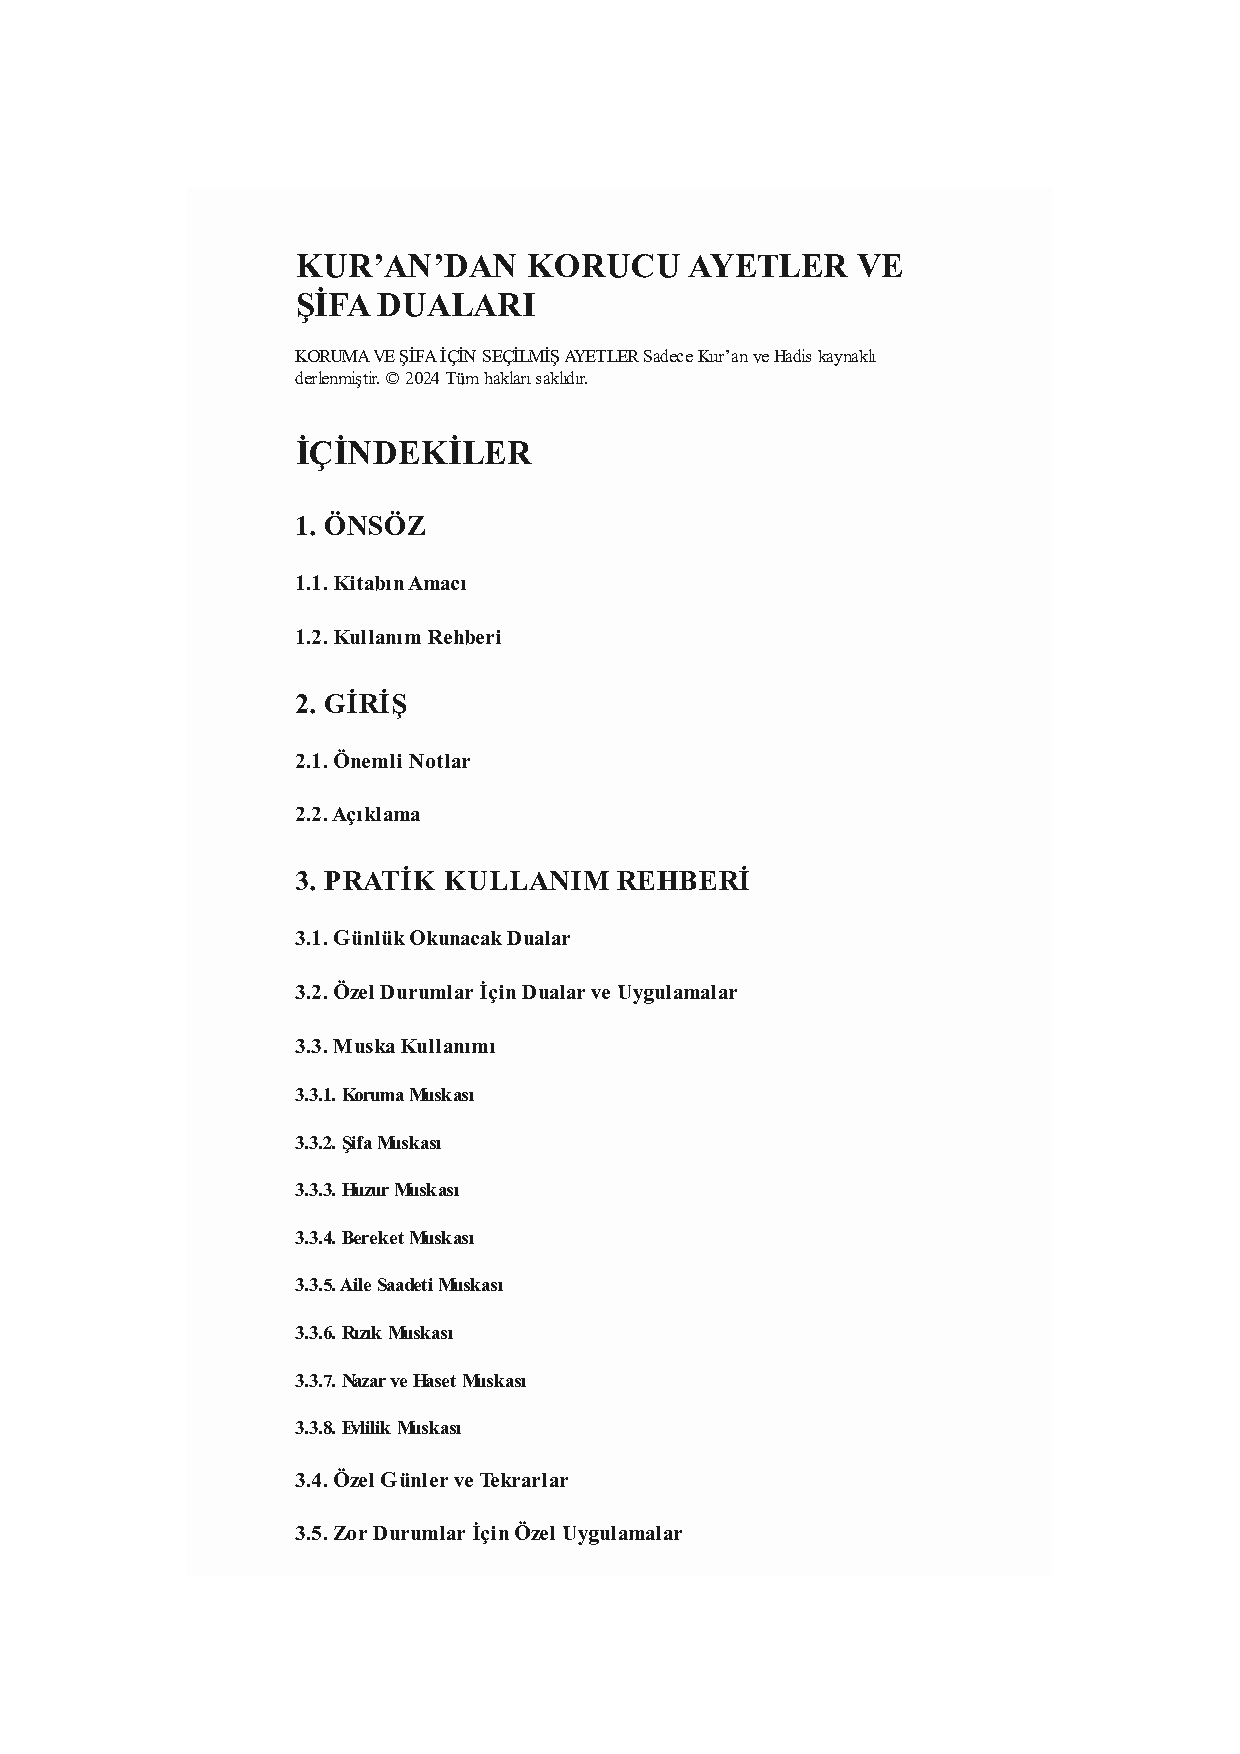
\includepdf[pages=-]{input/kitap.pdf}
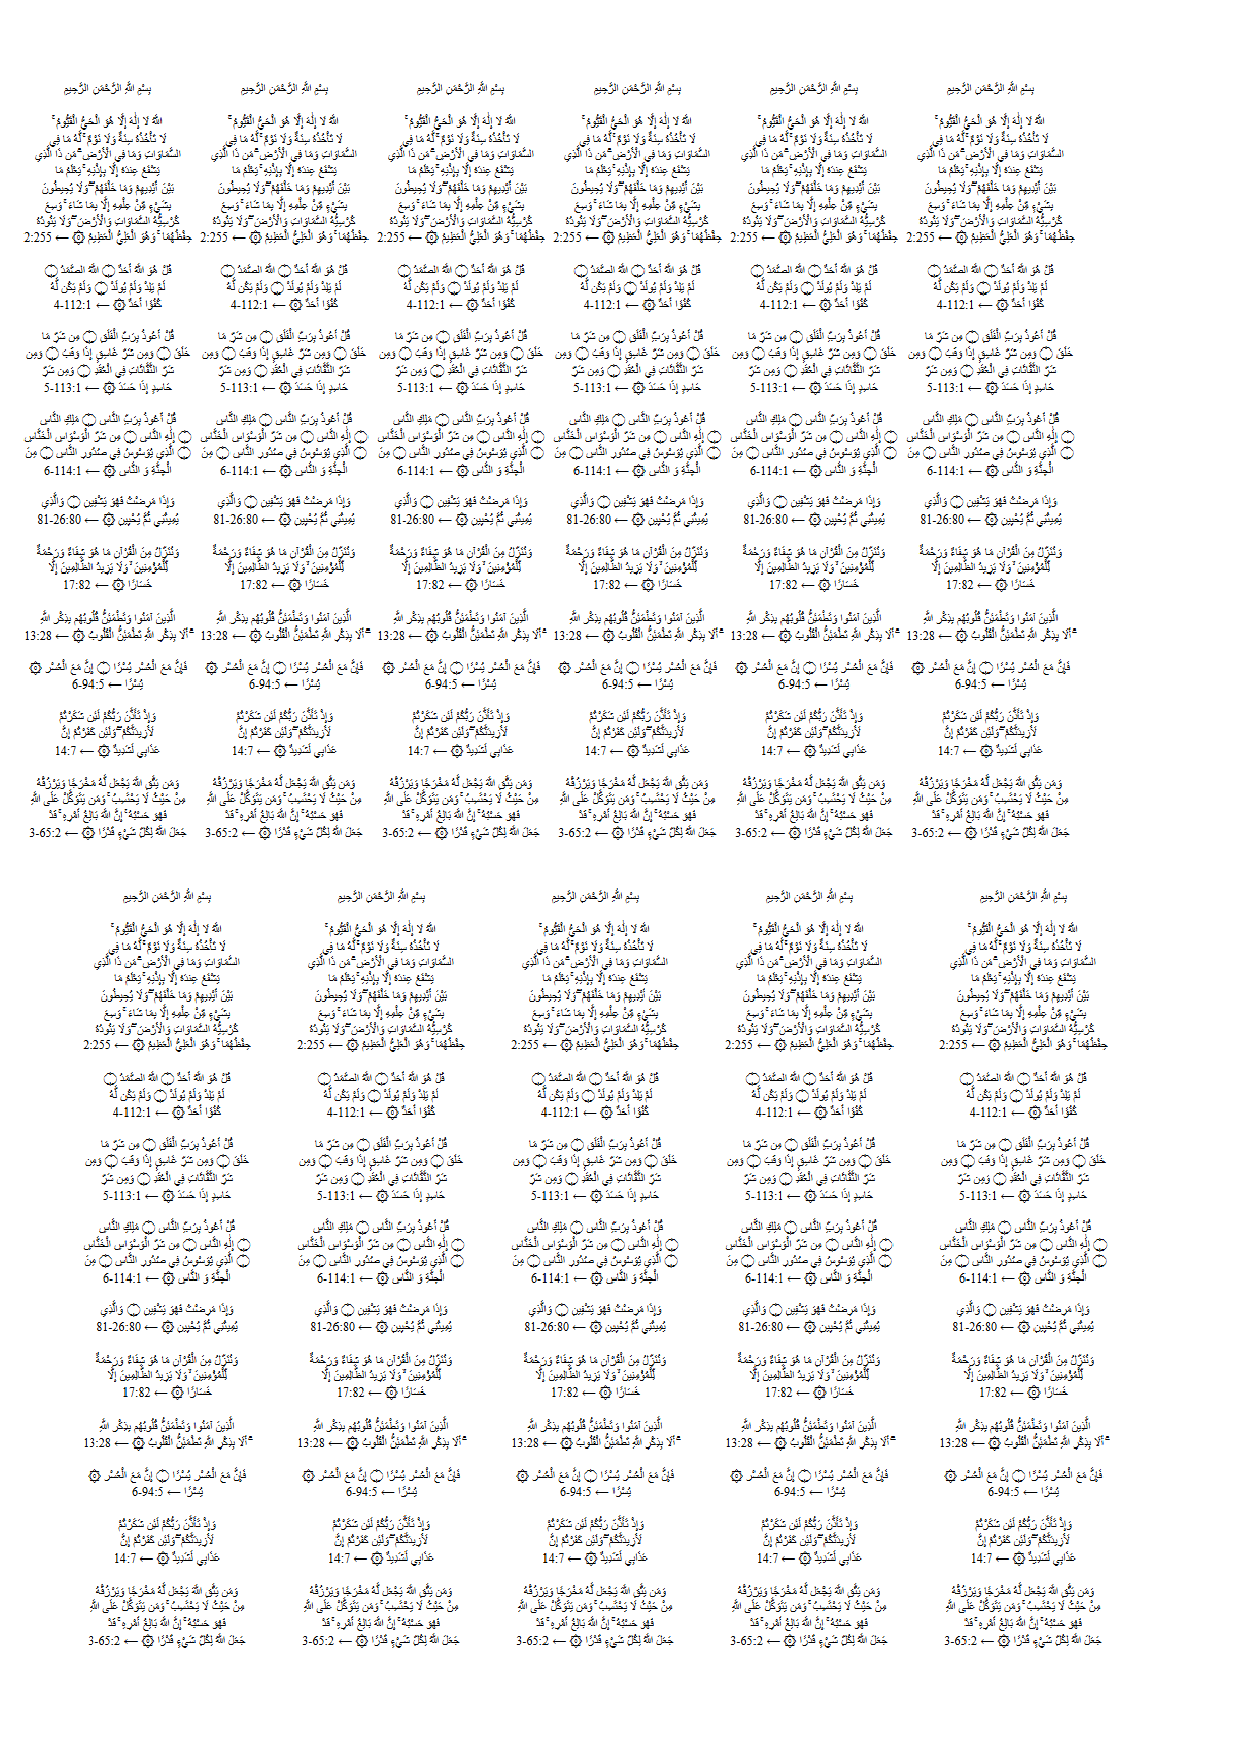
\includepdf[pages=-]{input/muska.pdf}

\end{document} 